% =====================================================================
%  Presentación de avance de tesis — Prof. Enrique Espina
%  Felipe Gajardo Ávalos · Magíster en Ciencias de la Ingeniería, USACH
%  Compilar: latexmk -pdf presentacion_tesis_espina.tex
% =====================================================================
\documentclass[aspectratio=169,11pt]{beamer}

% ---------------------------------------------------------------------
%  BLOQUE DE ESTILO (reemplazable por la plantilla de Circuitos I)
% ---------------------------------------------------------------------
\usetheme{default}
\usefonttheme{professionalfonts}
\definecolor{usachA}{HTML}{00305E}   % azul institucional (ajustar)
\definecolor{usachB}{HTML}{EA7600}   % naranjo institucional (ajustar)
\definecolor{grisT}{HTML}{4A4A4A}
\definecolor{faseA}{HTML}{C0392B}
\definecolor{faseB}{HTML}{2E8B57}
\definecolor{faseC}{HTML}{1F5FAF}
\definecolor{ctrl}{HTML}{D35400}
\setbeamercolor{structure}{fg=usachA}
\setbeamercolor{frametitle}{fg=white,bg=usachA}
\setbeamercolor{title}{fg=usachA}
\setbeamercolor{subtitle}{fg=usachB}
\setbeamercolor{normal text}{fg=grisT}
\setbeamercolor{alerted text}{fg=usachB}
\setbeamercolor{block title}{fg=white,bg=usachA}
\setbeamercolor{block body}{bg=usachA!6}
\setbeamercolor{block title alerted}{fg=white,bg=usachB}
\setbeamercolor{block body alerted}{bg=usachB!8}
\setbeamertemplate{navigation symbols}{}
\setbeamertemplate{itemize items}[circle]
\setbeamertemplate{blocks}[rounded]
\setbeamertemplate{frametitle}{%
  \nointerlineskip\begin{beamercolorbox}[wd=\paperwidth,ht=2.4ex,dp=1.2ex,leftskip=1em]{frametitle}%
  \usebeamerfont{frametitle}\insertframetitle\end{beamercolorbox}%
  \nointerlineskip\hbox{\color{usachB}\rule{\paperwidth}{1.2pt}}}
\setbeamertemplate{footline}{%
  \leavevmode\hbox{\begin{beamercolorbox}[wd=\paperwidth,ht=2.5ex,dp=1ex]{normal text}%
  \hspace{1em}\scriptsize\color{usachA}F. Gajardo Ávalos · Tesis de Magíster · USACH%
  \hfill\insertframenumber\,/\,\inserttotalframenumber\hspace{1em}\end{beamercolorbox}}}
% ---------------------------------------------------------------------

\usepackage[utf8]{inputenc}
\usepackage[T1]{fontenc}
% En un TeX completo (TeX Live / MiKTeX / Overleaf) descomentar la línea siguiente:
% \usepackage[spanish,es-nodecimaldot,es-noshorthands]{babel}
\usepackage[scaled=.92]{helvet}   % Helvetica (Type 1) para el texto
\usepackage{amsmath,amssymb,bm}
\usepackage{booktabs,array,tabularx}
\usepackage{graphicx}
\usepackage{tikz}
\usetikzlibrary{arrows.meta,positioning,calc,fit,backgrounds}
\graphicspath{{fig/}}

% Notación
\newcommand{\Pic}[1]{P_{\mathrm{IC},#1}}
\newcommand{\Picr}[1]{P^{*}_{\mathrm{IC},#1}}
\newcommand{\Pnet}[1]{P_{\mathrm{net},#1}}
\newcommand{\Pbat}[1]{P_{\mathrm{B},#1}}
\newcommand{\Pnetm}{\bar P_{\mathrm{net}}}
\newcommand{\SOC}[1]{\mathrm{SOC}_{#1}}
\newcommand{\SOCw}{\overline{\mathrm{SOC}}_{w}}
\newcommand{\dec}{{,}}

\tikzset{
  blk/.style={draw,rounded corners=2pt,minimum height=0.95cm,align=center,font=\footnotesize,line width=.5pt},
  ac/.style={blk,fill=gray!12},
  ic/.style={blk,fill=usachA!12,draw=usachA},
  dc/.style={blk,fill=faseB!10,draw=faseB!70!black},
  co/.style={blk,fill=ctrl!12,draw=ctrl},
  pw/.style={{Latex[length=2mm]}-{Latex[length=2mm]},line width=.7pt},
  sg/.style={-{Latex[length=2mm]},dashed,line width=.6pt,ctrl},
}

\title{Coordinación SOC-consciente de convertidores por fase\\en una Micro-red híbrida AC/DC trifásica de cuatro hilos}
\subtitle{Planteamiento del problema, formulación y resultados preliminares}
\author{Felipe Gajardo Ávalos}
\institute{Magíster en Ciencias de la Ingeniería, mención Eléctrica\\Departamento de Ingeniería Eléctrica · Universidad de Santiago de Chile\\[2pt]Profesor guía: Dr. Enrique Espina González}
\date{Octubre de 2026}

\begin{document}

% ---------------------------------------------------------------------
\begin{frame}[plain]
  \titlepage
\end{frame}

% ---------------------------------------------------------------------
\begin{frame}{Contenido}
  \begin{columns}[T]
    \column{.48\textwidth}
    \begin{enumerate}
      \item Contexto y motivación
      \item Arquitectura propuesta
      \item Nomenclatura y supuestos
      \item Modelo energético por fase
      \item El problema: desbalance originado en DC
      \item Métricas de desbalance
      \item Formulación y brecha de la literatura
    \end{enumerate}
    \column{.48\textwidth}
    \begin{enumerate}\setcounter{enumi}{7}
      \item Ley de coordinación SOC-consciente
      \item Propiedades de la ley
      \item Implementación distribuida (consenso)
      \item Resultados preliminares
      \item Problemas abiertos
      \item Hoja de ruta y decisiones
      \item Literatura recomendada
    \end{enumerate}
  \end{columns}
\end{frame}

% =====================================================================
\section{Contexto}
\begin{frame}{1. Contexto y motivación}
  \begin{columns}[c]
    \column{.56\textwidth}
    \begin{itemize}\setlength\itemsep{4pt}
      \item Las redes de distribución BT son \textbf{trifásicas de cuatro hilos} (3$\phi$-4W) y alimentan cargas monofásicas fase--neutro.
      \item Los recursos distribuidos (FV, BESS, EV/V2G) son nativamente \textbf{DC} y crecen de forma \textbf{asimétrica} entre fases.
      \item Integrar recursos DC \textbf{por fase}, con un convertidor monofásico (IC) por fase, permite una expansión modular\ldots
      \item \ldots pero cada fase intercambia con la red una potencia distinta: aparece \alert{corriente de neutro} y desbalance en el PCC.
    \end{itemize}
    \column{.42\textwidth}
    \begin{alertblock}{Pregunta de investigación}
      \small ¿Cómo coordinar tres Micro-redes DC independientes, conectadas por fase, para reducir el desbalance visto por la red sin violar las restricciones de SOC de cada fase?
    \end{alertblock}
  \end{columns}
\end{frame}

% =====================================================================
\section{Arquitectura}
\begin{frame}{2. Arquitectura propuesta}
  \centering
  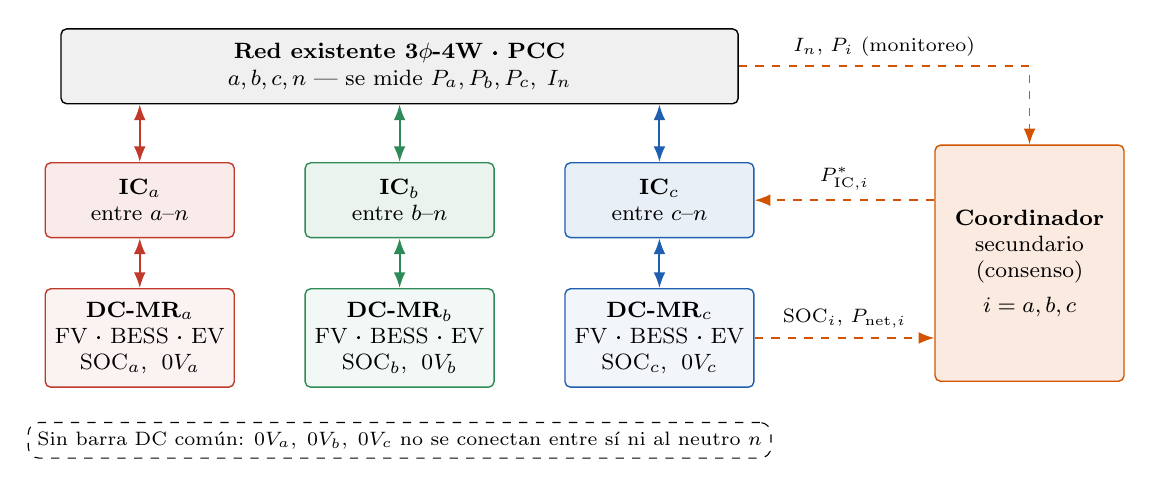
\begin{tikzpicture}[x=1cm,y=1cm]
    \node[ac,minimum width=8.6cm] (red) at (3.3,3.3) {\textbf{Red existente 3$\phi$-4W · PCC} \\ $a,b,c,n$ — se mide $P_a,P_b,P_c,\;I_n$};
    \foreach \x/\f/\c in {0/a/faseA,3.3/b/faseB,6.6/c/faseC}{
      \node[ic,minimum width=2.4cm,draw=\c,fill=\c!10] (ic\f) at (\x,1.6) {\textbf{IC}$_\f$ \\ entre $\f$--$n$};
      \node[dc,minimum width=2.4cm,minimum height=1.25cm,draw=\c,fill=\c!6] (dc\f) at (\x,-0.15) {\textbf{DC-MR}$_\f$ \\ FV · BESS · EV \\ $\SOC{\f}$,\; $0V_\f$};
      \draw[pw,\c] (ic\f.north) -- (ic\f.north |- red.south);
      \draw[pw,\c] (ic\f.south) -- (dc\f.north);
    }
    \node[co,minimum width=2.4cm,minimum height=3.0cm] (co) at (11.3,0.8) {\textbf{Coordinador} \\ secundario \\ (consenso) \\[3pt] $i=a,b,c$};
    \draw[sg] (red.east) -| node[pos=.25,above,font=\scriptsize,black]{$I_n$, $P_i$ (monitoreo)} (co.north);
    \draw[sg] (co.west |- icc) -- node[above,font=\scriptsize,black]{$\Picr{i}$} (icc.east);
    \draw[sg] (dcc.east) -- node[above,font=\scriptsize,black]{$\SOC{i},\,\Pnet{i}$} (co.west |- dcc);
    \node[draw,dashed,rounded corners,font=\scriptsize,align=center,minimum width=8.6cm] at (3.3,-1.45) {Sin barra DC común: $0V_a,\;0V_b,\;0V_c$ no se conectan entre sí ni al neutro $n$};
  \end{tikzpicture}

  \vspace{2pt}
  {\scriptsize Línea continua: potencia (bidireccional). Línea discontinua: señales de medición y referencia.}
\end{frame}

\begin{frame}{2. Detalle de una rama (fase $i$) y jerarquía de control}
  \begin{columns}[T]
    \column{.5\textwidth}
    \centering\textbf{\small Etapas de potencia}\\[3pt]
    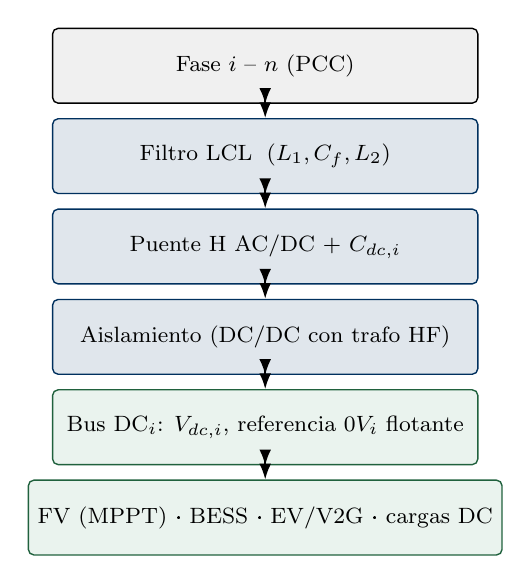
\begin{tikzpicture}[node distance=0.18cm,every node/.append style={minimum height=0.56cm}]
      \node[ac,minimum width=5.4cm] (g) {Fase $i$ -- $n$ (PCC)};
      \node[ic,minimum width=5.4cm,below=of g] (f) {Filtro LCL \;($L_1,C_f,L_2$)};
      \node[ic,minimum width=5.4cm,below=of f] (h) {Puente H AC/DC + $C_{dc,i}$};
      \node[ic,minimum width=5.4cm,below=of h] (iso) {Aislamiento (DC/DC con trafo HF)};
      \node[dc,minimum width=5.4cm,below=of iso] (bus) {Bus DC$_i$: $V_{dc,i}$, referencia $0V_i$ flotante};
      \node[dc,minimum width=5.4cm,below=of bus] (r) {FV (MPPT) · BESS · EV/V2G · cargas DC};
      \foreach \u/\v in {g/f,f/h,h/iso,iso/bus,bus/r}{\draw[pw] (\u.south) -- (\v.north);}
    \end{tikzpicture}
    \column{.5\textwidth}
    \centering\textbf{\small Capas de control y escalas de tiempo}\\[3pt]
    \scriptsize
    \begin{tabular}{@{}lll@{}}
      \toprule
      Capa & Función & Escala \\ \midrule
      Corriente del IC & PR a 50 Hz + PLL, PWM & ms \\
      Potencia del IC & sigue $\Picr{i}$ & 10--100 ms \\
      BESS (primario DC) & forma $V_{dc,i}$ (droop $V$--$P$) & 10--100 ms \\
      \alert{Coordinador} & consenso + ley SOC & s -- min \\
      Dinámica del SOC & constante $\tau$ & horas \\ \bottomrule
    \end{tabular}

    \vspace{4pt}
    \begin{block}{Decisión de modelado}
      \scriptsize En el caso coordinado la \textbf{BESS forma el bus DC} y el IC opera como fuente de potencia que sigue $\Picr{i}$. Si el IC regulara $V_{dc,i}$, perdería el grado de libertad para obedecer al coordinador.
    \end{block}
  \end{columns}
\end{frame}

% =====================================================================
\section{Nomenclatura}
\begin{frame}{3. Nomenclatura}
  \scriptsize\renewcommand{\arraystretch}{1.12}
  \begin{columns}[T]
    \column{.49\textwidth}
    \begin{tabular}{@{}lll@{}}
      \toprule
      Símbolo & Descripción & Unidad \\ \midrule
      $i\in\{a,b,c\}$ & fase / agente & -- \\
      $\Pnet{i}$ & potencia neta de la DC-MR$_i$ & kW \\
      $P_{\mathrm{load},i}$ & carga DC de la fase $i$ & kW \\
      $P_{\mathrm{EV},i}$ & carga del vehículo eléctrico & kW \\
      $P_{\mathrm{PV},i}$ & generación fotovoltaica & kW \\
      $\Pic{i}$ & potencia del IC ($>0$: red $\to$ DC) & kW \\
      $\Picr{i}$ & referencia de potencia del IC & kW \\
      $\Pbat{i}$ & potencia de la BESS ($>0$: descarga) & kW \\
      $\SOC{i}$ & estado de carga de la BESS & p.u. \\
      $E_i$ & capacidad nominal de la BESS & kWh \\
      $\tau$ & constante de tiempo de coordinación & h \\ \bottomrule
    \end{tabular}
    \column{.49\textwidth}
    \begin{tabular}{@{}lll@{}}
      \toprule
      Símbolo & Descripción & Unidad \\ \midrule
      $\Pnetm$ & promedio de las $\Pnet{i}$ & kW \\
      $\SOCw$ & SOC promedio ponderado por $E_i$ & p.u. \\
      $V$ & tensión fase--neutro eficaz & V \\
      $I_n$ & corriente de neutro en el PCC & A \\
      $I_0,\,I_1,\,I_2$ & secuencias cero, positiva y negativa & A \\
      VUF, CUF & factores de desbalance (tensión, corriente) & \% \\
      $\mathcal{N}_i$ & vecinos del agente $i$ & -- \\
      $\bm L$ & laplaciano del grafo de comunicación & -- \\
      $x_{P,i},\,x_{ES,i},\,x_{E,i}$ & estados de consenso del agente $i$ & -- \\
      $\varepsilon$ & ganancia de consenso & -- \\
      $D$ & dispersión de potencias por fase & kW \\ \bottomrule
    \end{tabular}
  \end{columns}
\end{frame}

\begin{frame}{3. Supuestos del modelo energético (nivel 1)}
  \begin{enumerate}\setlength\itemsep{3pt}
    \item Red \textbf{rígida}: tensiones fase--neutro balanceadas de módulo $V=230$ V y $Z_{\mathrm{red}}=0$.
    \item IC con \textbf{factor de potencia unitario} y sin pérdidas; dinámica eléctrica despreciable frente a la del SOC.
    \item El bus DC no almacena energía en la escala de minutos: $C_{dc}\,V_{dc}\,\dot V_{dc}\approx 0$.
    \item \textbf{No existe camino DC entre fases}: la energía solo pasa de una fase a otra a través de la red AC.
    \item Paso de simulación de 1 min; 4 días con perfiles diarios repetidos; se reporta el día 4 (régimen periódico).
  \end{enumerate}
  \vspace{4pt}
  \begin{block}{Parámetros del escenario}
    \footnotesize $E_i=20$ kWh · $\SOC{i}\in[0{,}1;\,0{,}9]$ · $|\Pbat{i}|\le 5$ kW · $|\Pic{i}|\le 12$ kW · cargas 1{,}4/1{,}0/0{,}8 p.u. · FV pico 0/1{,}5/3{,}0 kW · EV 3{,}7 kW en fase $a$ (19--21 h).
  \end{block}
\end{frame}

% =====================================================================
\section{Modelo}
\begin{frame}{4. Modelo energético por fase}
  \begin{columns}[c]
    \column{.5\textwidth}
    \textbf{Potencia neta de la DC-MR$_i$}
    \begin{equation}
      \Pnet{i} = P_{\mathrm{load},i} + P_{\mathrm{EV},i} - P_{\mathrm{PV},i}
    \end{equation}
    \textbf{Balance del bus DC}
    \begin{equation}
      \Pic{i} + \Pbat{i} = \Pnet{i}
    \end{equation}
    \textbf{Dinámica del SOC}
    \begin{equation}
      E_i\,\frac{d\,\SOC{i}}{dt} = -\Pbat{i} = \Pic{i} - \Pnet{i}
    \end{equation}
    {\footnotesize El IC y la BESS son ``vasos comunicantes'': lo que no trae el IC lo entrega la batería, y eso tiene memoria.}
    \column{.48\textwidth}
    \centering
    \includegraphics[width=\linewidth]{Pnet.pdf}\\
    {\scriptsize Potencia neta por fase (día tipo). Medias diarias: 1{,}65 / 0{,}54 / $-$0{,}07 kW.}
  \end{columns}
\end{frame}

% =====================================================================
\section{Problema}
\begin{frame}{5. El problema: el desbalance se origina en el lado DC}
  \begin{columns}[c]
    \column{.55\textwidth}
    Con FP unitario y tensión balanceada, $\vec I_i = (P_i/V)\angle\theta_i$ y
    \begin{equation}
      |I_n| = |\vec I_a+\vec I_b+\vec I_c| = 3|I_0| = \frac{D}{V}
    \end{equation}
    \vspace{-10pt}
    \begin{align*}
      D&=\sqrt{P_a^2+P_b^2+P_c^2-P_aP_b-P_bP_c-P_cP_a}\\
       &=\sqrt{\tfrac32\textstyle\sum_i (P_i-\bar P)^2}
    \end{align*}
    \vspace{-4pt}
    \begin{itemize}\scriptsize\setlength\itemsep{1pt}
      \item $I_n=0 \iff P_a=P_b=P_c$: mide cuánto \textbf{se separan} las fases, no cuánto consumen.
      \item Con control local, $\Pic{i}=\Pnet{i}$: la red ve directamente la asimetría de los recursos DC.
      \item Ej. 20:00 h: $7{,}2/2{,}5/2{,}0$ kW $\Rightarrow D=4{,}97$ kW $\Rightarrow |I_n|=21{,}6$ A.
    \end{itemize}
    \column{.43\textwidth}
    \centering
    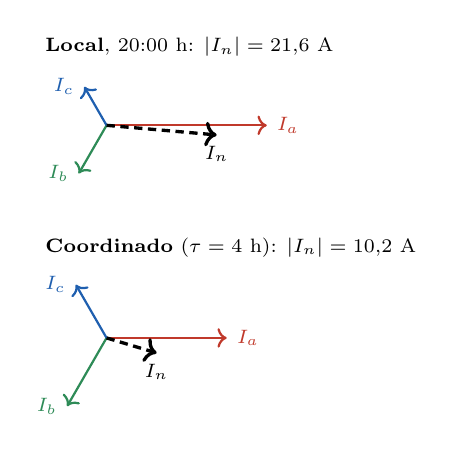
\begin{tikzpicture}[scale=1]
      \def\k{0.065}
      \begin{scope}
        \node[font=\scriptsize,anchor=west] at (-0.9,1.0) {\textbf{Local}, 20:00 h: $|I_n|=21{,}6$ A};
        \draw[->,faseA,thick] (0,0) -- (0:{31.30*\k}) node[right,font=\scriptsize]{$I_a$};
        \draw[->,faseB,thick] (0,0) -- (-120:{10.87*\k}) node[left,font=\scriptsize]{$I_b$};
        \draw[->,faseC,thick] (0,0) -- (120:{8.70*\k}) node[left,font=\scriptsize]{$I_c$};
        \draw[->,black,very thick,densely dashed] (0,0) -- ({21.52*\k},{-1.879*\k}) node[below,font=\scriptsize]{$I_n$};
      \end{scope}
      \begin{scope}[yshift=-2.7cm]
        \node[font=\scriptsize,anchor=west] at (-0.9,1.15) {\textbf{Coordinado} ($\tau=4$ h): $|I_n|=10{,}2$ A};
        \draw[->,faseA,thick] (0,0) -- (0:{23.48*\k}) node[right,font=\scriptsize]{$I_a$};
        \draw[->,faseB,thick] (0,0) -- (-120:{15.39*\k}) node[left,font=\scriptsize]{$I_b$};
        \draw[->,faseC,thick] (0,0) -- (120:{12.0*\k}) node[left,font=\scriptsize]{$I_c$};
        \draw[->,black,very thick,densely dashed] (0,0) -- ({9.78*\k},{-2.94*\k}) node[below,font=\scriptsize]{$I_n$};
      \end{scope}
    \end{tikzpicture}\\[2pt]
    {\scriptsize Fasores a escala; $I_n$ en línea discontinua.}
  \end{columns}
\end{frame}

\begin{frame}{6. Métricas de desbalance (componentes simétricas)}
  \begin{columns}[T]
    \column{.52\textwidth}
    \begin{equation*}
      \begin{bmatrix}X_0\\X_1\\X_2\end{bmatrix}=\frac13
      \begin{bmatrix}1&1&1\\1&a&a^2\\1&a^2&a\end{bmatrix}
      \begin{bmatrix}X_a\\X_b\\X_c\end{bmatrix},\quad a=1\angle120^\circ
    \end{equation*}
    \begin{align}
      \mathrm{VUF} &= \frac{|V_2|}{|V_1|}\cdot100\,\%, & \mathrm{VUF}_0 &= \frac{|V_0|}{|V_1|}\cdot100\,\% \\
      \mathrm{CUF}_2 &= \frac{|I_2|}{|I_1|}\cdot100\,\%, & \mathrm{CUF}_0 &= \frac{|I_0|}{|I_1|}\cdot100\,\%
    \end{align}
    Relación causa--efecto: \;$V_2\approx Z_2 I_2$, \;\; $V_0\approx (Z_{\mathrm{f}}+3Z_n)\,I_0$.
    \column{.45\textwidth}
    \begin{alertblock}{Consecuencias para esta tesis}
      \footnotesize
      \begin{itemize}
        \item Con red rígida ($Z=0$) el \textbf{VUF es nulo por construcción}: se evaluará en el nivel 2 (PLECS con impedancia de red).
        \item Con FP unitario: $\mathrm{CUF}_0=\mathrm{CUF}_2=D/\sum_i P_i$, que \textbf{diverge} cuando $\sum P_i\to0$ (mediodía con FV).
        \item Métrica principal: $|I_n|$ en A (RMS, pico, p95). CUF normalizado a $I_{\mathrm{nom}}$.
        \item Límite de referencia VUF: 2\,\% (EN 50160 / NTCS, verificar vigencia).
      \end{itemize}
    \end{alertblock}
  \end{columns}
\end{frame}

% =====================================================================
\section{Formulación}
\begin{frame}{7. Formulación del problema de coordinación}
  \begin{columns}[T]
    \column{.55\textwidth}
    \textbf{Variables de decisión:} $\Picr{a},\Picr{b},\Picr{c}$ en cada instante.
    \begin{align*}
      \min_{\Picr{i}}\quad & J=\int_0^T |I_n(t)|^2\,dt \\
      \text{s.a.}\quad & E_i\,\dot{\mathrm{SOC}}_i = \Pic{i}-\Pnet{i} \\
      & \mathrm{SOC}_{\min}\le\SOC{i}\le\mathrm{SOC}_{\max} \\
      & |\Pbat{i}|\le P_{\mathrm{B},\max},\quad |\Pic{i}|\le P_{\mathrm{IC},\max} \\
      & \text{información local + vecinos (sin coordinador central)}
    \end{align*}
    \column{.42\textwidth}
    \begin{alertblock}{Restricción estructural: piso energético}
      \footnotesize En régimen periódico el SOC vuelve a su valor inicial, luego
      \[\textstyle\int_{\mathrm{día}}\Pic{i}\,dt=\int_{\mathrm{día}}\Pnet{i}\,dt .\]
      La componente media diaria del desbalance \textbf{no puede eliminarse} con baterías por fase:
      \[ I_{n,\mathrm{RMS}} \;\ge\; \frac{D\big(\langle\Pnet{i}\rangle_{\mathrm{día}}\big)}{V} = 6{,}6\ \mathrm{A}\]
      {\scriptsize con medias diarias 1{,}65 / 0{,}54 / $-$0{,}07 kW.}
      La batería solo desplaza energía \textbf{en el tiempo}, no entre fases.
    \end{alertblock}
  \end{columns}
\end{frame}

\begin{frame}{7. Brecha en la literatura}
  \footnotesize
  \begin{tabularx}{\textwidth}{@{}p{3.3cm}X p{3.4cm}@{}}
    \toprule
    Línea & Qué resuelve & Qué no cubre \\ \midrule
    Desbalance en Micro-redes AC de 3 y 4 hilos (droop por fase, CPT, consenso) [5,6] & Reparto de corrientes desbalanceadas entre convertidores \textbf{AC} & El origen está en cargas AC; no hay DC por fase \\
    Micro-redes híbridas con IC [1,10,13] & Coordinación AC global -- DC global mediante \textbf{un} IC (agente de consenso) & Un solo bus DC compartido; sin asimetría por fase \\
    Balance de SOC en Micro-redes DC [11,12] & Igualar SOC entre BESS de \textbf{un mismo} bus DC & Las BESS comparten bus: la energía fluye entre ellas \\ \midrule
    \alert{Esta tesis} & \multicolumn{2}{p{9.6cm}}{Desbalance \textbf{originado en el lado DC} por tres DC-MR independientes; el SOC de cada fase es el único grado de libertad y no hay camino DC entre fases. No se identificó este planteamiento en la revisión realizada.} \\ \bottomrule
  \end{tabularx}

  \vspace{6pt}
  \normalsize Extensión directa de la tesis doctoral del Prof. Espina: de \textbf{un} IC como agente de consenso a \textbf{tres} IC asociados a fases.
\end{frame}

% =====================================================================
\section{Ley}
\begin{frame}{8. Ley de coordinación SOC-consciente}
  \begin{equation}
    \boxed{\;\Picr{i} \;=\; \underbrace{\Pnetm}_{\text{balance}} \;+\; \underbrace{\frac{E_i}{\tau}\big(\SOCw-\SOC{i}\big)}_{\text{corrección por SOC}}\;},\qquad i=a,b,c
  \end{equation}
  \vspace{-4pt}
  \[
    \Pnetm=\tfrac13\textstyle\sum_j \Pnet{j},\qquad
    \SOCw=\dfrac{\sum_j E_j\,\SOC{j}}{\sum_j E_j}
  \]
  \begin{columns}[T]
    \column{.5\textwidth}
    \begin{itemize}\footnotesize
      \item \textbf{Balance:} todas las fases piden lo mismo $\Rightarrow I_n\to0$.
      \item \textbf{Corrección:} la fase con batería bajo el promedio pide más a la red y descarga menos; la que está sobre el promedio, pide menos.
      \item $E_i/\tau$: ganancia [kW/p.u.]. Con 20 kWh y 4 h: 5 kW/p.u.
    \end{itemize}
    \column{.48\textwidth}
    \begin{itemize}\footnotesize
      \item $\tau\to0$: control local (la batería no actúa).
      \item $\tau\to\infty$: balance puro, sin SOC (las baterías saturan).
      \item $\tau$ es la perilla entre ambos extremos.
    \end{itemize}
  \end{columns}
\end{frame}

\begin{frame}{8. Ejemplo numérico de un instante}
  \centering\footnotesize
  $E_i=20$ kWh, $\tau=4$ h $\Rightarrow E_i/\tau = 5$ kW/p.u. \qquad $\Pnetm=1{,}0$ kW, \quad $\SOCw=0{,}50$\\[6pt]
  \begin{tabular}{lccc}
    \toprule
    & Fase $a$ & Fase $b$ & Fase $c$ \\ \midrule
    $\Pnet{i}$ [kW] & 4{,}0 & 1{,}0 & $-$2{,}0 \\
    $\SOC{i}$ [p.u.] & 0{,}30 & 0{,}55 & 0{,}65 \\
    Corrección $5(\SOCw-\SOC{i})$ [kW] & $+$1{,}00 & $-$0{,}25 & $-$0{,}75 \\
    $\Picr{i}$ [kW] & \textbf{2{,}00} & \textbf{0{,}75} & \textbf{0{,}25} \\
    $\Pbat{i}=\Pnet{i}-\Pic{i}$ [kW] & 2{,}00 (desc.) & 0{,}25 (desc.) & $-$2{,}25 (carga) \\ \bottomrule
  \end{tabular}\\[8pt]
  \begin{tabular}{lcc}
    \toprule
    Estrategia & Potencias vistas por la red [kW] & $|I_n|$ [A] \\ \midrule
    Local & 4{,}0 / 1{,}0 / $-$2{,}0 & 22{,}6 \\
    Balance sin SOC & 1{,}0 / 1{,}0 / 1{,}0 & 0 \;(pero BESS$_a$ al 30\,\% descarga 3 kW) \\
    \alert{Con SOC} & 2{,}0 / 0{,}75 / 0{,}25 & 6{,}8 \\ \bottomrule
  \end{tabular}
\end{frame}

% =====================================================================
\section{Propiedades}
\begin{frame}{9. Propiedades de la ley}
  \footnotesize
  \begin{columns}[T]
    \column{.5\textwidth}
    \textbf{P1. Conservación}
    \[\textstyle\sum_i \Picr{i}=\sum_i \Pnet{i}\]
    {\footnotesize La ley no cambia la energía total intercambiada con la red; solo la redistribuye entre fases.}

    \vspace{4pt}
    \textbf{P2. Equivalencia con filtro de primer orden} {\footnotesize($E_i$ iguales, sin saturación)}
    \begin{equation}
      \tau\,\frac{d\,\Delta\Pic{i}}{dt}+\Delta\Pic{i}=\Delta\Pnet{i}
    \end{equation}
    \vspace{-10pt}
    \[\Leftrightarrow\quad \Delta\Pic{i}(s)=\frac{\Delta\Pnet{i}(s)}{1+s\tau}\]
    {\footnotesize La red ve la parte lenta del desbalance; la BESS absorbe la rápida: $\Pbat{i}(s)=\frac{s\tau}{1+s\tau}\Delta\Pnet{i}(s)$.}
    \column{.48\textwidth}
    \textbf{P3. Piso energético:} la componente DC del desbalance pasa intacta por el filtro $\Rightarrow$ 6{,}6 A.

    \vspace{6pt}
    \textbf{P4. Regla de diseño de $\tau$}
    \[|\SOC{i}-\SOCw|\approx\frac{\tau\,|\Delta\Pnet{i}|}{E_i}\le m\]
    \vspace{-6pt}
    \[\Rightarrow\quad \tau\le\frac{E_i\,m}{|\Delta\Pnet{i}|_{\max}}\]
    {\footnotesize $m$: margen de SOC disponible. Fase $a$: $\Delta=0{,}94$ kW, $\tau=4$ h $\Rightarrow$ desviación 0{,}19; predice $\SOC{a}\approx31\,\%$, simulación 28\,\%.}

    \vspace{6pt}
    \textbf{P5. Falla sin SOC:} con $\tau\to\infty$ la batería de la fase deficitaria se agota en el primer día y el sistema vuelve al caso local.
  \end{columns}
\end{frame}

% =====================================================================
\section{Consenso}
\begin{frame}{10. Implementación distribuida: consenso de promedio dinámico}
  \begin{columns}[T]
    \column{.52\textwidth}
    Cada agente estima los promedios globales con información local y de sus vecinos:
    \begin{equation}
      x_i \leftarrow x_i-\varepsilon\sum_{j\in\mathcal N_i}(x_i-x_j),\qquad 0<\varepsilon<\frac{2}{\lambda_{\max}(\bm L)}
    \end{equation}
    {\footnotesize Corrección dinámica previa: $x_i\leftarrow x_i + (u_i[k]-u_i[k-1])$, para seguir señales variables [9].}
    \begin{equation*}
      \Picr{i}=x_{P,i}+\frac{E_i}{\tau}\left(\frac{x_{ES,i}}{x_{E,i}}-\SOC{i}\right)
    \end{equation*}
    {\footnotesize $x_{P,i}\to\Pnetm$, \; $x_{ES,i}\to\mathrm{prom}(E\cdot\mathrm{SOC})$, \; $x_{E,i}\to\mathrm{prom}(E)$.}
    \column{.45\textwidth}
    \centering
    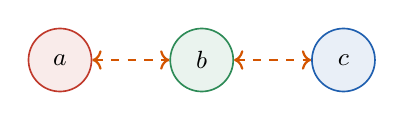
\begin{tikzpicture}[ag/.style={circle,draw,minimum size=8mm,font=\small,line width=.6pt}]
      \node[ag,draw=faseA,fill=faseA!10] (a) at (0,0) {$a$};
      \node[ag,draw=faseB,fill=faseB!10] (b) at (1.8,0) {$b$};
      \node[ag,draw=faseC,fill=faseC!10] (c) at (3.6,0) {$c$};
      \draw[<->,dashed,ctrl,thick] (a) -- (b); \draw[<->,dashed,ctrl,thick] (b) -- (c);
    \end{tikzpicture}\\[4pt]
    \footnotesize
    $\bm L=\begin{bmatrix}1&-1&0\\-1&2&-1\\0&-1&1\end{bmatrix}$, \quad $\lambda(\bm L)=\{0,\,1,\,3\}$\\[4pt]
    $\varepsilon<2/3$; con $\varepsilon=0{,}3$: $\rho=\max|1-\varepsilon\lambda|=0{,}7$ por iteración.\\[3pt]
    10 iteraciones/paso $\Rightarrow$ error $0{,}7^{10}\approx2{,}8\,\%$.\\[3pt]
    \alert{Distribuido vs. centralizado: error máx. 0{,}053 kW.}
  \end{columns}
\end{frame}

\begin{frame}{10. Estructura interna del agente $i$}
  \centering
  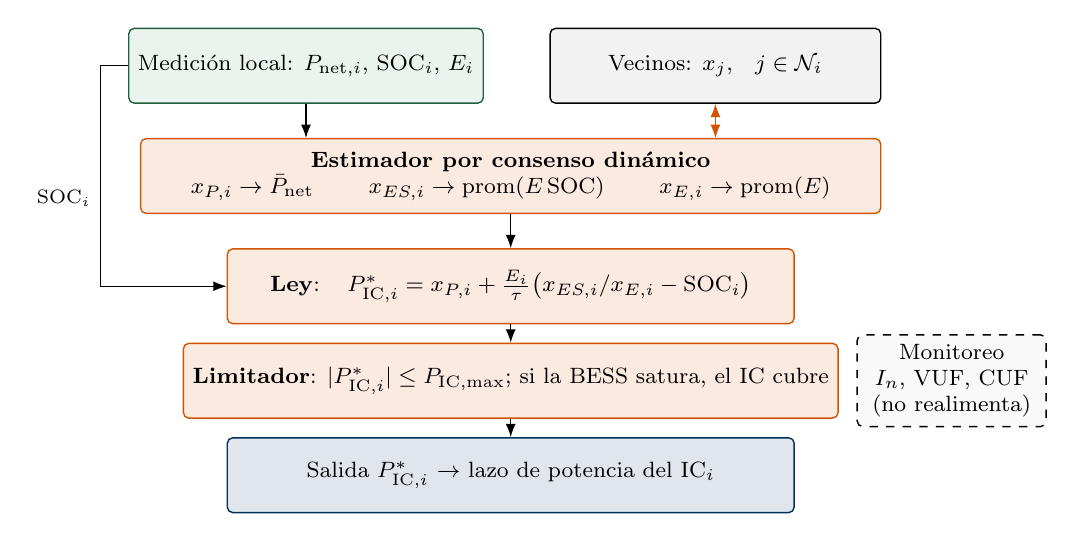
\begin{tikzpicture}[x=1cm,y=1cm,every node/.append style={minimum height=0.8cm}]
    \node[dc,minimum width=4.2cm] (m) at (-2.6,3.0) {Medición local: $\Pnet{i}$, $\SOC{i}$, $E_i$};
    \node[blk,fill=gray!10,minimum width=4.2cm] (v) at (2.6,3.0) {Vecinos: $x_j$, \; $j\in\mathcal N_i$};
    \node[co,minimum width=9.4cm,align=center] (est) at (0,1.6) {\textbf{Estimador por consenso dinámico}\\ $x_{P,i}\to\Pnetm$ \qquad $x_{ES,i}\to\mathrm{prom}(E\,\mathrm{SOC})$ \qquad $x_{E,i}\to\mathrm{prom}(E)$};
    \node[co,minimum width=7.2cm] (ley) at (0,0.2) {\textbf{Ley}: \; $\Picr{i}=x_{P,i}+\frac{E_i}{\tau}\big(x_{ES,i}/x_{E,i}-\SOC{i}\big)$};
    \node[co,minimum width=7.2cm] (lim) at (0,-1.0) {\textbf{Limitador}: $|\Picr{i}|\le P_{\mathrm{IC},\max}$; si la BESS satura, el IC cubre};
    \node[ic,minimum width=7.2cm] (out) at (0,-2.2) {Salida $\Picr{i}$ $\to$ lazo de potencia del IC$_i$};
    \node[blk,dashed,fill=gray!5,minimum width=2.4cm,align=center] (mon) at (5.6,-1.0) {Monitoreo\\$I_n$, VUF, CUF\\(no realimenta)};
    \draw[-{Latex}] (m.south) -- (m.south |- est.north);
    \draw[{Latex}-{Latex},dashed,ctrl] (v.south) -- (v.south |- est.north);
    \draw[-{Latex}] (est) -- (ley); \draw[-{Latex}] (ley) -- (lim); \draw[-{Latex}] (lim) -- (out);
    \draw[-{Latex}] (m.west) -- ++(-0.35,0) |- node[pos=.3,left,font=\scriptsize]{$\SOC{i}$} (ley.west);
  \end{tikzpicture}
\end{frame}

% =====================================================================
\section{Resultados}
\begin{frame}{11. Resultados preliminares: corriente de neutro}
  \begin{columns}[c]
    \column{.6\textwidth}
    \includegraphics[width=\linewidth]{In_dia4.pdf}
    \column{.38\textwidth}
    \footnotesize
    \begin{tabular}{@{}lccc@{}}
      \toprule
      Estrategia & RMS & Pico & SOC \\
       & [A] & [A] & [\%] \\ \midrule
      Local & 8{,}8 & 21{,}6 & 50--50 \\
      Sin SOC & 8{,}8 & 21{,}6 & 10--90 \\
      \alert{SOC, $\tau=4$ h} & \alert{7{,}2} & \alert{12{,}6} & 12--76 \\
      Distribuido & 7{,}2 & 12{,}6 & 12--76 \\ \bottomrule
    \end{tabular}\\[6pt]
    \begin{itemize}
      \item Pico de $I_n$: $-42\,\%$.
      \item Sin SOC: 12\,824 min$\cdot$fase de saturación en 4 días.
      \item Con SOC: sin saturación.
    \end{itemize}
  \end{columns}
\end{frame}

\begin{frame}{11. Resultados preliminares: SOC y elección de $\tau$}
  \begin{columns}[T]
    \column{.52\textwidth}
    \centering
    \includegraphics[width=\linewidth]{SOC.pdf}\\
    {\scriptsize Sin SOC: $\SOC{a}\to10\,\%$ y $\SOC{b},\SOC{c}\to90\,\%$ en el primer día. Con SOC: ciclo diario estable (fin de día $\approx$ 28/56/65\,\%).}
    \column{.46\textwidth}
    \centering
    \includegraphics[width=\linewidth]{tau_sweep.pdf}\\
    \tiny\setlength\tabcolsep{3pt}
    \begin{tabular}{@{}lccccccc@{}}
      \toprule
      $\tau$ [h] & 1 & 2 & 3 & \textbf{4} & 5 & 6 & 8 \\ \midrule
      Pico $|I_n|$ [A] & 19{,}1 & 15{,}7 & 13{,}8 & \textbf{12{,}6} & 17{,}9 & 19{,}8 & 20{,}0 \\
      SOC mín [\%] & 35 & 26 & 19 & \textbf{12} & 10 & 10 & 10 \\
      Saturación [min$\cdot$fase] & 0 & 0 & 0 & \textbf{0} & 71 & 205 & 1163 \\ \bottomrule
    \end{tabular}\\[3pt]
    \scriptsize $\tau=4$ h: mayor valor sin saturación y menor pico.
  \end{columns}
\end{frame}

% =====================================================================
\section{Problemas abiertos}
\begin{frame}{12. Problemas abiertos}
  \footnotesize
  \begin{tabularx}{\textwidth}{@{}p{3.6cm}X@{}}
    \toprule
    Problema & Situación y consecuencia \\ \midrule
    1. Sin transferencia DC entre fases & Piso de 6{,}6 A en el escenario: límite físico de la arquitectura, no del control. \\
    2. Modelo de red rígida & VUF $\equiv$ 0. Requiere $Z_s$, $Z_n$ (nivel 2): $v_{pcc,i}=e_i+Z_s i_i - Z_n(i_a+i_b+i_c)$. \\
    3. Compensación con $Q$ & A las 20:00, $Q=-0{,}29/3{,}0/-2{,}71$ kvar anula $I_0$ (7{,}2$\to$0 A) pero eleva $I_2$ (7{,}2$\to$14{,}4 A): traslada el desbalance a secuencia negativa. \\
    4. ¿Quién forma $V_{dc,i}$? & IC (caso base del documento) vs. BESS (modelo y ley). Debe fijarse explícitamente. \\
    5. Rizado a $2\omega$ del IC monofásico & $C_{dc}\ge P/(\omega V_{dc}\Delta V_{pp})$: 5 kW, 400 V, 1\,\% $\Rightarrow\approx$ 9{,}9 mF, o filtro/notch activo. \\
    6. Aislamiento galvánico & Garantiza $0V_i\ne n$; agrega un convertidor por fase (costo y pérdidas). \\
    7. Alcance EV/V2G & ¿Núcleo de la tesis o extensión? \\
    8. Comunicación & Retardos y pérdida de enlaces en el consenso; robustez a falla de un agente. \\ \bottomrule
  \end{tabularx}
\end{frame}

% =====================================================================
\section{Hoja de ruta}
\begin{frame}{13. Hoja de ruta de simulación y validación}
  \centering
  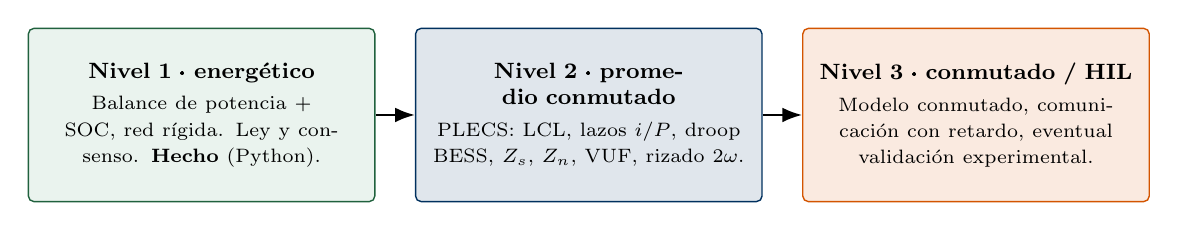
\begin{tikzpicture}[node distance=0.5cm]
    \node[dc,minimum width=4.4cm,minimum height=2.2cm,text width=4.1cm] (n1) {\textbf{Nivel 1 · energético}\\[2pt]\scriptsize Balance de potencia + SOC, red rígida. Ley y consenso. \textbf{Hecho} (Python).};
    \node[ic,minimum width=4.4cm,minimum height=2.2cm,text width=4.1cm,right=of n1] (n2) {\textbf{Nivel 2 · promedio conmutado}\\[2pt]\scriptsize PLECS: LCL, lazos $i$/$P$, droop BESS, $Z_s$, $Z_n$, VUF, rizado $2\omega$.};
    \node[co,minimum width=4.4cm,minimum height=2.2cm,text width=4.1cm,right=of n2] (n3) {\textbf{Nivel 3 · conmutado / HIL}\\[2pt]\scriptsize Modelo conmutado, comunicación con retardo, eventual validación experimental.};
    \draw[-{Latex[length=2.5mm]},thick] (n1) -- (n2); \draw[-{Latex[length=2.5mm]},thick] (n2) -- (n3);
  \end{tikzpicture}

  \vspace{10pt}
  \begin{columns}[T]
    \column{.48\textwidth}
    \textbf{Casos de estudio}
    \begin{itemize}\footnotesize
      \item Equilibrado; carga / FV / SOC desigual.
      \item EV monofásico y V2G.
      \item Saturación de convertidor y pérdida de un recurso.
      \item Falla de un enlace de comunicación.
    \end{itemize}
    \column{.48\textwidth}
    \textbf{Comparación}
    \begin{itemize}\footnotesize
      \item Local vs. balance sin SOC vs. SOC-consciente.
      \item Centralizado vs. distribuido.
      \item Métricas: $|I_n|$ (RMS, pico, p95), VUF, CUF$_{\mathrm{nom}}$, excursión SOC, saturación, pérdidas.
    \end{itemize}
  \end{columns}
\end{frame}

\begin{frame}{13. Decisiones para conversar}
  \begin{enumerate}\setlength\itemsep{5pt}
    \item ¿Es correcta la topología con el neutro solo en el dominio AC y referencias DC flotantes, con o sin aislamiento galvánico?
    \item ¿Centrar el aporte en la \textbf{coordinación SOC-consciente por fase} y no en una nueva topología de convertidor?
    \item Piso de desbalance por diferencias de energía diaria: ¿se declara como límite físico o se incorpora otro grado de libertad ($Q$, carga flexible)?
    \item Validación: ¿coordinador centralizado primero y luego consenso, o directamente distribuido?
    \item ¿EV/V2G en el núcleo o como extensión?
    \item ¿Plataforma experimental disponible (prototipo de laboratorio) para el nivel 3?
  \end{enumerate}
\end{frame}

% =====================================================================
\section{Literatura}
\begin{frame}{14. Literatura recomendada: mapa de lectura}
  \footnotesize\renewcommand{\arraystretch}{1.25}
  \begin{tabularx}{\textwidth}{@{}p{3.0cm}X p{2.6cm}@{}}
    \toprule
    Para entender\ldots & Pregunta que responde & Referencias \\ \midrule
    \textbf{El enfoque} & ¿Qué es el control jerárquico y cómo se separan primario, secundario y terciario? ¿Por qué distribuido? & [2], [3] \\
    & ¿Cómo converge el consenso y cómo se sigue un promedio que cambia en el tiempo? & [4], [9], [7] \\
    \textbf{El problema} & ¿Cómo se mide y comparte el desbalance en Micro-redes de 3 y 4 hilos? & [5], [6], [14], [15] \\
    & ¿Qué hace un IC en una Micro-red híbrida y cómo se coordina con ambos lados? & [10], [13] \\
    \textbf{La solución} & ¿Cómo entra el IC como agente de consenso? (base que se extiende a tres IC) & [1] \\
    & ¿Cómo se balancea el SOC con control distribuido? & [11], [12], [8] \\ \bottomrule
  \end{tabularx}

  \vspace{8pt}
  \textbf{Orden sugerido:} [2] $\to$ [3] $\to$ [4], [9] $\to$ [1] $\to$ [5], [6] $\to$ [11], [12] $\to$ [10], [13] $\to$ [14].
\end{frame}

\begin{frame}{14. Literatura recomendada (1/2)}
  \scriptsize
  \textbf{Control jerárquico y consenso}
  \begin{itemize}\setlength\itemsep{1pt}
    \item[{[1]}] E. Espina, R. Cárdenas-Dobson, D. Sáez, M. Kazerani, J. W. Simpson-Porco, ``A consensus-based secondary control strategy for hybrid ac/dc microgrids with experimental validation,'' \emph{IEEE Trans. Power Electron.}, vol.~36, no.~5, pp.~5971--5984, 2021. \alert{Base metodológica directa.}
    \item[{[2]}] E. Espina, J. Llanos, C. Burgos-Mellado, R. Cárdenas-Dobson, M. Martínez-Gómez, D. Sáez, ``Distributed control strategies for microgrids: An overview,'' \emph{IEEE Access}, vol.~8, pp.~193412--193448, 2020. \alert{Mapa del área.}
    \item[{[3]}] J. M. Guerrero, J. C. Vasquez, J. Matas, L. G. de Vicuña, M. Castilla, ``Hierarchical control of droop-controlled AC and DC microgrids,'' \emph{IEEE Trans. Ind. Electron.}, vol.~58, no.~1, pp.~158--172, 2011.
    \item[{[4]}] R. Olfati-Saber, J. A. Fax, R. M. Murray, ``Consensus and cooperation in networked multi-agent systems,'' \emph{Proc. IEEE}, vol.~95, no.~1, pp.~215--233, 2007.
    \item[{[9]}] S. S. Kia, B. Van Scoy, J. Cortés, R. A. Freeman, K. M. Lynch, S. Martínez, ``Tutorial on dynamic average consensus,'' \emph{IEEE Control Syst. Mag.}, vol.~39, no.~3, pp.~40--72, 2019. \alert{Fundamento del estimador.}
    \item[{[7]}] J. W. Simpson-Porco \emph{et al.}, ``Secondary frequency and voltage control of islanded microgrids via distributed averaging,'' \emph{IEEE Trans. Ind. Electron.}, vol.~62, no.~11, pp.~7025--7038, 2015.
  \end{itemize}
  \textbf{Métricas de desbalance}
  \begin{itemize}\setlength\itemsep{1pt}
    \item[{[14]}] P. Pillay, M. Manyage, ``Definitions of voltage unbalance,'' \emph{IEEE Power Eng. Rev.}, vol.~21, no.~5, pp.~50--51, 2001.
    \item[{[15]}] EN 50160 / IEC 61000-4-30 y Norma Técnica de Calidad de Servicio para Sistemas de Distribución (Chile) --- límites de VUF (verificar versión vigente).
  \end{itemize}
\end{frame}

\begin{frame}{14. Literatura recomendada (2/2)}
  \scriptsize
  \textbf{Desbalance en sistemas de tres y cuatro hilos}
  \begin{itemize}\setlength\itemsep{1pt}
    \item[{[5]}] C. Burgos-Mellado, J. Llanos, E. Espina \emph{et al.}, ``Single-phase consensus-based control for regulating voltage and sharing unbalanced currents in 3-wire isolated AC microgrids,'' \emph{IEEE Access}, vol.~8, pp.~164882--164898, 2020.
    \item[{[6]}] C. Burgos-Mellado \emph{et al.}, ``Distributed control strategy based on a consensus algorithm and on the conservative power theory for imbalance and harmonic sharing in 4-wire microgrids,'' \emph{IEEE Trans. Smart Grid}, vol.~11, no.~2, pp.~1604--1619, 2020.
  \end{itemize}
  \textbf{Micro-redes híbridas e interlinking converters}
  \begin{itemize}\setlength\itemsep{1pt}
    \item[{[10]}] P. C. Loh, D. Li, Y. K. Chai, F. Blaabjerg, ``Autonomous operation of hybrid microgrid with AC and DC subgrids,'' \emph{IEEE Trans. Power Electron.}, vol.~28, no.~5, pp.~2214--2223, 2013.
    \item[{[8]}] V. Nasirian, S. Moayedi, A. Davoudi, F. L. Lewis, ``Distributed cooperative control of DC microgrids,'' \emph{IEEE Trans. Power Electron.}, vol.~30, no.~4, pp.~2288--2303, 2015.
    \item[{[13]}] M. Najafzadeh \emph{et al.}, ``Recent contributions, future prospects and limitations of interlinking converter control in hybrid AC/DC microgrids,'' \emph{IEEE Access}, vol.~9, 2021.
  \end{itemize}
  \textbf{Balance de SOC}
  \begin{itemize}\setlength\itemsep{1pt}
    \item[{[11]}] X. Lu, K. Sun, J. M. Guerrero, J. C. Vasquez, L. Huang, ``State-of-charge balance using adaptive droop control for distributed energy storage systems in DC microgrid applications,'' \emph{IEEE Trans. Ind. Electron.}, vol.~61, no.~6, pp.~2804--2815, 2014.
    \item[{[12]}] T. Morstyn, B. Hredzak, V. G. Agelidis, ``Cooperative multi-agent control of heterogeneous storage devices distributed in a DC microgrid,'' \emph{IEEE Trans. Power Syst.}, vol.~31, no.~4, pp.~2974--2986, 2016.
  \end{itemize}
\end{frame}

% ---------------------------------------------------------------------
\begin{frame}[plain]
  \centering\vfill
  {\Large\color{usachA}\textbf{Síntesis}}\\[10pt]
  \begin{minipage}{.82\textwidth}\centering
    La ley convierte a cada batería en un \textbf{filtro pasa altos del desbalance}: absorbe lo rápido y no puede absorber el promedio.\\[6pt]
    De ahí salen el \alert{beneficio} ($-42\,\%$ en el pico de $I_n$), el \alert{límite} (piso de 6{,}6 A) y la \alert{regla de diseño} ($\tau\approx4$ h).
  \end{minipage}
  \vfill
  {\small Felipe Gajardo Ávalos · felipe.gajardo.a@usach.cl}
  \vfill
\end{frame}

\end{document}
